\documentclass[11pt,letterpaper]{article}
\usepackage{naaclhlt2010}
\usepackage{times}
\usepackage{graphicx}
\usepackage{latexsym}
\setlength\titlebox{6.5cm}    % Expanding the titlebox

\title{EN.600.461 Computer Vision\\Final Project\\Recognizing and Translating Text from Images}

\author{Joon Hyuck (James) Choi\\
  (Senior Undergraduate)\\
  The Johns Hopkins University\\
  3400 N Charles Street\\
  Baltimore, MD 21218, USA\\
  {\tt jchoi100@jhu.edu}}

\date{Dec X, 2016}

\begin{document}
\maketitle
\begin{abstract}
  This work explores optical character recognition (OCR) in photos of printed and hand-written documents. It first explores basic preprocessing of photos of documents using {\tt OpenCV} \footnote{http://opencv.org/} functionalities for blurring, thresholding, and denoising. It next discusses the use of {\tt tesseract-ocr} \footnote{https://github.com/tesseract-ocr} to perform OCR. We then discuss the incorporation of the Google Cloud Translation API \footnote{https://cloud.google.com/translate/} to translate the OCR results to different languages. If finally discusses template matching using the Johns Hopkins University (JHU) logo. 
\end{abstract}

\section{Introduction}

This work achieved the following main goals stated in the original project proposal: 1) Given a photo of a document, convert it into a clean scanned version; 2) Take the scanned version and perform OCR. Optionally, this work took the OCR output and translated the text into different languages using the Google Cloud Translation API. This work also experimented with template matching using the JHU logo in order to determine whether the input document is an official JHU document or not.

\section{Methods}

In this section, we discuss the methods we took and external libraries used for each stage of our work.

\subsection{Image Preprocessing}

We implemented our program in Python using {\tt OpenCV}. In order to feed the OCR algorithm clean input to achieve best performance, we used {\tt cv2.medianBlur} to smoothen the input image with an aperture size of 5. Then, we passed the smoothened image through {\tt cv2.adaptiveThreshold} with \textit{adaptiveMethod=} {\tt ADAPTIVE\textunderscore THRESH\textunderscore GAUSSIAN\textunderscore C}, \textit{threshold = binary}, \textit{blockSize=5x5}, and \textit{C=2}. The adaptive method we chose uses the weighted sum of the \textit{blockSize} x \textit{blockSize neighborhood of pixel (x, y) - C} as its threshold value. Parameter values were chosen empirically.

Finally, we performed denoising on the thresholded image to remove noise and make the output clean. We used {\tt cv2.fastNlMeansDenoising} with \textit{templateWindowSize=7}, \textit{searchWindowSize = 21}, and \textit{h=7}. Numbers here were also chosen empirically. The motivation behind denoising in our work was that document scans usually have many random specs here and there. Such noise can greatly reduce OCR accuracy because an OCR algorithm may confuse a random spec with punctuation marks or associate a spec with an actual character near by (e.g. confuse an $l$ with an $i$).

\subsection{OCR}

In order to perform OCR on the cleaned inputs, we used the {\tt tesseract-ocr} library through its python wrapper {\tt pytesseract}. We used the raw output from {\tt pytesseract}'s {\tt image\textunderscore to\textunderscore string} method to pass into python's file writer and Google Cloud Translation API.

As a side experiment, we used the {\tt Keras} \footnote{https://keras.io/} library to train the MNIST \footnote{http://yann.lecun.com/exdb/mnist/} dataset of 70,000 handwritten digits on three different convolutional neural networks (CNN). Results will be discussed in section 3.3. We referred to code online \footnote{http://machinelearningmastery.com/handwritten-digit-recognition-using-convolutional-neural-networks-python-keras/} to build the three CNNs.

\subsection{Translation}

We made use of Google Cloud's Translation API in order to translate the OCR processed document into several different languages based on user command line input. We referred to code posted online \footnote{http://github.com/mouuff/mtranslate} and modified the details to fit our purpose.

\subsection{Template Matching}

Aside from OCR, which was the main focus of this project, we experimented with template matching in images. Specifically, we used the JHU logo to determine whether the input document was an official JHU document or not. We naively assumed that official JHU documents contained a JHU logo for our experiment's sake. We used {\tt cv2.matchTemplate} with our input document as the source image, multiple JHU logo images (each with different sizes since {\tt cv2.matchTemplate} is scale sensitive) as templates, and matching method {\tt cv2.TM\textunderscore CCOEFF\textunderscore NORMED}. If the normazlied {\tt TM\textunderscore CCOEFF} value came out to be greater than 0.51 for any of the input JHU logo templates of various sizes, we determined that the input document contained a JHU logo in it. The matching method and determinant value of 0.51 were chosen empirically.

\section{Results}

Here, we qualitatively discuss OCR results on typed and handwritten input documents.

\subsection{Typed Documents}

We ran our code on five document images with different font types and sizes: {\tt cv\textunderscore proj\textunderscore description.png}, {\tt aesop\textunderscore fox.png}, {\tt aesop\textunderscore miller.png}, {\tt aesop\textunderscore goose.png}, {\tt aesop\textunderscore cat.png}. With the exception of {\tt aesop\textunderscore goose.png}, performance on all documents were near-perfect. A sample image is shown in Figure 1.

\begin{figure}[t!]
  \centering
  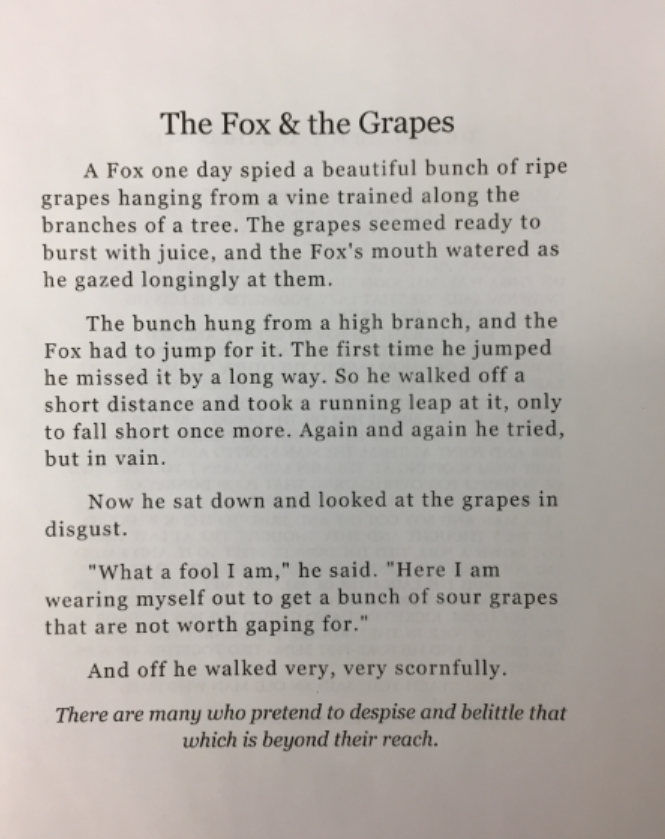
\includegraphics[keepaspectratio, width=0.5\textwidth]{fox.png}
  \caption{Sample typed document in our dataset}
\end{figure}

We ran our code on additional two document images that were taken under sub-optimal conditions: irregular lighting, partial skew, and/or laminated surfaces. These images were {\tt cv\textunderscore jchoi\textunderscore proposal.png} and {\tt jhu\textunderscore lav\textunderscore notes1.png}. Despite the less optimal environment, our code was able to correctly denoise and threshold the images and gave similar results as before.

\subsection{Handwritten Documents}

\subsection{MNIST Training with Keras}

\begin{figure}[t!]
  \centering
  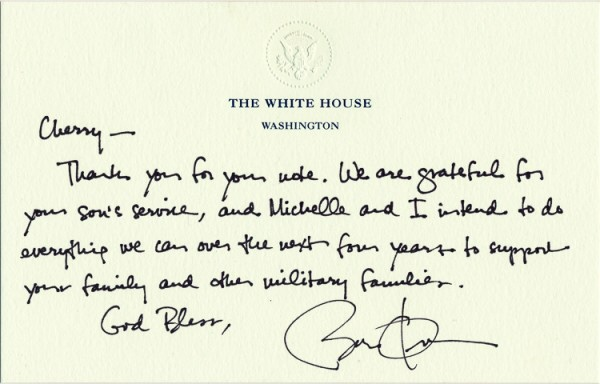
\includegraphics[keepaspectratio, width=0.5\textwidth]{obama4.png}
  \caption{Sample handwritten document in our dataset}
\end{figure}



\section{Discussion}

\section{How to Run the Code}

Please extract {\tt FINAL\textunderscore PROJECT\textunderscore jchoi100.zip} to view and run the code.

Assuming that the user has Python 2.5+, OpenCV, pytesseract, and tesseract installed, run the following command on the command line in the same directory as {\tt driver.py}.

{\tt \$python driver.py \{path-to-image-} {\tt file\} \{list of target languages separated by single space\}}\\

\textbf{Sample usage:}

{\tt \$python driver.py data/doc7.png es fr}

performs OCR on {\tt doc7.png}, outputs the thresholded image, the text in the original input language, and the text translated in Spanish and French.


\begin{itemize}
\item Left and right margins: 1in
\item Top margin:1in
\item Bottom margin: 1in
\item Column width: 3.15in
\item Column height: 9in
\item Gap between columns: 0.2in
\end{itemize}


\begin{table}
\begin{center}
\begin{tabular}{|l|rl|}
\hline \bf Type of Text & \bf Font Size & \bf Style \\ \hline
paper title & 15 pt & bold \\
author names & 12 pt & bold \\
author affiliation & 12 pt & \\
the word ``Abstract'' & 12 pt & bold \\
section titles & 12 pt & bold \\
document text & 11 pt  &\\
abstract text & 10 pt & \\
captions & 10 pt & \\
bibliography & 10 pt & \\
footnotes & 9 pt & \\
\hline
\end{tabular}
\end{center}
\caption{\label{font-table} Font guide. }
\end{table}

{\bf Captions}: Provide a caption for every illustration; number each one
sequentially in the form:  ``Figure 1. Caption of the Figure.'' ``Table 1.
Caption of the Table.''  Type the captions of the figures and 
tables below the body, using 10 point text.  

\section*{Acknowledgments}

We thank the python libraries we used for image processing and OCR, the code we referred to for constructing CNNs using {\tt Keras} and making use of the Google Translate API, and MNIST for the handwritten digit dataset.

\end{document}
